\documentclass[a4paper,11pt]{article}
\usepackage[T1]{fontenc}
\usepackage[english]{babel}
\usepackage[utf8]{inputenc}
\usepackage[a4paper, total={6in, 9in}]{geometry}
\usepackage{makeidx}
\usepackage{booktabs}  
\usepackage{graphicx} 
\usepackage{listings}
\usepackage[flushleft]{threeparttable}
\usepackage{hyperref}
\usepackage{float}
\usepackage{caption}
% \usepackage{subcaption}
%\usepackage[colorinlistoftodos]{todonotes}
\usepackage{amsmath}
\usepackage{siunitx}
\usepackage[dvipsnames]{xcolor}
\usepackage{tikz,lipsum,lmodern}
\usepackage[most]{tcolorbox}
\usepackage{biblatex} 
\addbibresource{sample.bib} 
\usepackage{indentfirst} 
\usepackage{subfigure}

%----------------------------------------------------------------------------------------
% Edita cabeçalho e rodapé
%----------------------------------------------------------------------------------------

\usepackage{fancyhdr}
\pagestyle{fancy}
\fancyhf{}

\usepackage{verbatim}
\hypersetup{
    colorlinks=true,
    linkcolor=blue,
    filecolor=blue,      
    urlcolor=blue,
    bookmarks=true,
    % pdfpagemode=FullScreen,
    } 
    
\lhead{
\begin{minipage}{5cm}\vspace{-1.4cm}\hspace{-1cm} 

\includegraphics[width=1.0\linewidth]{header}
% \includegraphics[width=0.2\linewidth]{lnls.png}
\end{minipage}}
\chead{LNLS/SIRIUS \\ Accelerator Physics Group - FAC }
\rhead{\today}
% \lfoot{}
\cfoot{\thepage}
\renewcommand{\headrulewidth}{1pt}
\renewcommand{\footrulewidth}{1pt}

\begin{document}
\begin{center}
\LARGE{Nonlinear optics optimization at SIRIUS storage ring}  
\end{center}
\begin{abstract}
This document compiles the results of our attempts at online optimization of SIRIUS nonlinear optics so far. We have applied our own implementation of the Robust Conjugate Direction Search (RCDS)\footnote{Which is available \href{https://github.com/lnls-fac/apsuite/blob/589267dadd42e95b3da0093a8e03f5e7c9ae155d/apsuite/optimization/rcds.py}{here}.} algorithm to optimize the machine Dynamic Aperture (DA) by probing the Injection Efficiency. We also tried optimizing an objective consisting on the scalar combination of objective functions probing DA and momentum aperture (MA).
\end{abstract}
\section{The first online optimization attempt}
The parameter space (knobs) consisted on the strength of the SDA0, SDB0, SDP0, SFA0, SFB0, SFP0, SDA1, SDB1, SDP1, SDA3, SDB3, SDP3, SFA1, SFB1, SFP1 sextupole families. The SDA2, SDB2, SDP2 and SFA2, SFB2, SFP2 families were used keep chromaticity constant when varying the optimization knobs. This was implemented in the following manner: RCDS freely proposed strength variations to the knob families. For each proposed change in strength, the corresponding changes in chromaticity were estimated from a chromaticity jacobian matrix constructed from the model. To the "correction"~ families were applied the strengths needed to cancel these chromaticity changes. In this first attempt, we tested the optimization routine twice, with different objective functions to probe the dynamic aperture.
\subsection{Kick resilience optimization}
The first objective function adopted was the beam loss after dipolar kick from the pingers. The idea was to minimize the loss at a given kick, and progressively increase the kicks, probing larger acceptances. The BPMs acquisition was fired in synchrony with the dipole kick and beam-loss was calculated by comparing the sum-signal of the first 10 turns with the sum-signal of the last 10 turns. As for the strength of the dipole kick, we set a horizontal kick of $\Delta x^\prime = -0.760~ \unit{m rad}$, which rendered about 35 - 60\% of beam-loss . A vertical kick of $\Delta y^\prime = 0.03~\unit{m rad}$ was also fired.

\subsubsection{Results}
In the first iteration, beam loss dropped from 60\% to nearly 0\% (see Figure~\ref{beam_loss_hist}). In the beginning of the 2nd iteration, the objective function took negative values and we stopped the optimization run. The sextupole families configurations before and after the optimization, as well as their respective changes in strength are shown in Figure~\ref{beam_loss_sexts}. 

The beam-loss minimization significantly improved the beam's resiliency to dipole kicks. After the optimization, it was necessary to kick the beam at approximately $-0.850~\unit{m rad}$ to achieve a  30--40\% beam-loss rate.
\begin{figure}
    \centering
    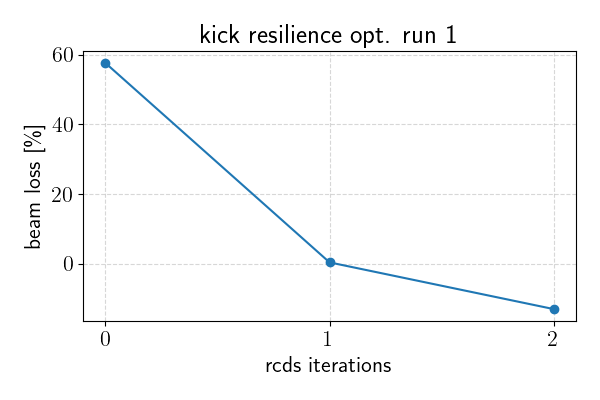
\includegraphics[scale=0.7]{beam_loss_hist_run1.png}
    \caption{Objective function history vs. iterations of the first trial at beam-loss optimization.}
    \label{beam_loss_hist}
\end{figure}
By the end of this first run, the machine magnets were cycled and the configurations found during optimization were reloaded. When trying to inject, the efficiency was quite low. The improved kick resilience, however, was preserved, which led to suspicion that the aperture along $-x$ might have been negatively impacted by the optimization, while the aperture in $x^\prime$ increased. This observation motivated the adoption of a different objective to probe the DA.

\begin{figure*}[t]
    \centering
    \includegraphics*[width=\textwidth]{beam_loss_sexts.png}
    \caption{Sextupole families strengths and strength changes before/after the beam-loss rate optimization}
    \label{beam_loss_sexts}
\end{figure*}

\subsection{Injection efficiency optimization}
Starting from the reference configurations (user's beam configurations), the injection conditions were worsened by reducing the NLK strength
%$-2.45~\unit{m rad}$ to $-2.25~\unit{m rad}$
. In the off-axis injection scheme, the reduction led the beam to be injected the upper left border of the  $(x,x^\prime)$ aperture (see Figure~\ref{fig:inj_cond}), and rendered an efficiency of about 30\%. The objective function adopted was the negative of the injection efficiency under these injection conditions. We hoped that minimizing this objective would correspond to a maximization of the DA more evenly among the $-x$ and $x^{\prime}$ directions.
\begin{figure}[h]
    \centering
    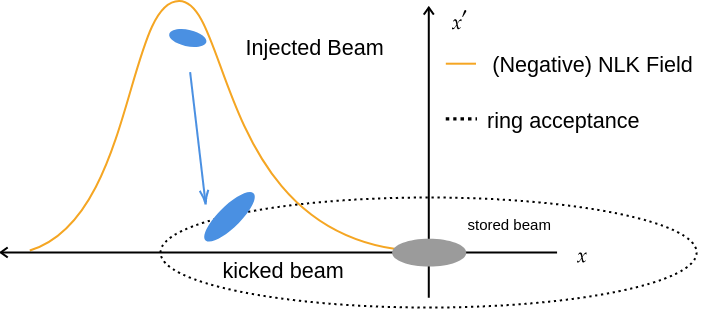
\includegraphics[width=0.7\columnwidth]{inj_cond.png}
    \caption{Injection conditions for DA optimization}
    \label{fig:inj_cond}
\end{figure}

\subsubsection{Results}
In the first run, within three iterations the injection efficiency reached 70\%. The algorithm stopped for achieving the maximum number of the objective function evaluations. We fired a second run, starting from the configurations just found. In four iterations we reached 85\% efficiency. When the NLK strength was restored to the reference value, meaning the nominal off-axis injection conditions were restored (in which the beam ``lands"~ within the acceptance), the injection efficiency fluctuated around 95--100\% with good repeatability. Beam lifetime by the end of the last optimization trial was 54.12 hrs at $15~\unit{mA}$ current. In the reference configuration optics, lifetime at this same current is about 68 hrs.
\begin{figure}[]
    \centering
    \begin{minipage}{0.48\textwidth}
        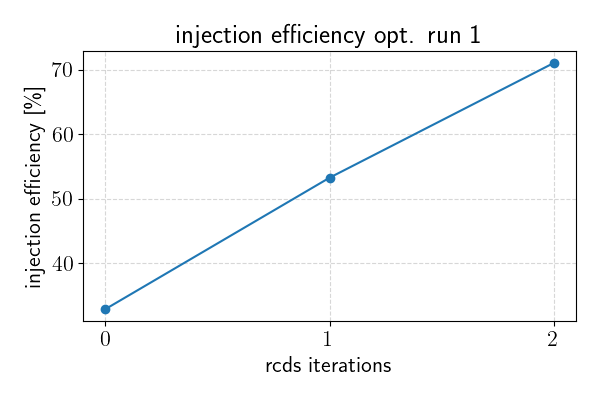
\includegraphics[width=\columnwidth]{injeff_hist_run1.png}
        \caption{Best obj. function during the 1st run of injection efficiency optimization}
        \label{injeff_hist1}  
    \end{minipage}%
    \hfill
    \begin{minipage}{0.48\textwidth}
        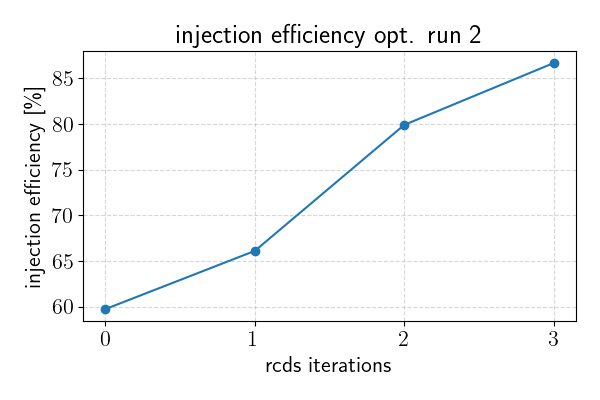
\includegraphics[width=\columnwidth]{injeff_hist_run2.png}
        \caption{Best obj. function during the 2nd run of injection efficiency optimization}
        \label{injeff_hist2}
    \end{minipage}
\end{figure}
The sextupole families strengths pre- and post-optimization, as well as the corresponding changes are presented by Figures~\ref{inject_sexts1} and ~\ref{inject_sexts2}, for the first and the second injection efficiency optimization runs, respectively.
\begin{figure*}[h]
    \centering
    \includegraphics*[width=1\textwidth]{sexts_injeff_run1.png}
    \caption{Sextupole families strengths and strength changes before/after the first run of injection efficiency optimization}
    \label{inject_sexts1}
\end{figure*}
\begin{figure*}[h]
    \centering
    \includegraphics*[width=\textwidth]{sexts_injeff_run2.png}
    \caption{Sextupole families strengths and strength changes before/after the first run of injection efficiency optimization}
    \label{inject_sexts2}
\end{figure*}

We carried out chromaticity measurements in the machine loaded with the reference configuration (ref-config) and with the sextupole configurations found at iterations 0, 2, and 3 of the last injection efficiency optimization run
(that of Figure~\ref{injeff_hist2}). Table~\ref{chrom} presents the measured values, from which one can notice a chromaticity drift. This drift probably arises from discrepancies between the model and the real machine, since the chromaticity "correction"~ depends on the chromaticity jacobian matrix built from the model.
\begin{table}[h]
\centering
\begin{tabular}{@{}ccc@{}}
\toprule
machine configuration & $\xi_x$       & $\xi_y$         \\ \midrule
ref-config   & $2.33\pm0.02$ & $2.531\pm0.008$ \\
iter 0   & $2.59\pm0.02$ & $3.700\pm0.008$   \\
iter 2   & $2.72\pm0.04$ & $3.704\pm0.008$ \\
iter 3   & $2.76\pm0.05$  & $3.510\pm0.01$   \\ \bottomrule
\end{tabular}
\caption{Chromaticity measurements for ref-config and sextupole configs. found at the second round of injection optimization}
\label{chrom}
\end{table}
Due to schedule limitations, we could to cycle the magnets and re-load the configurations found during optimization to check if the injection efficiency and lifetime would agree with the values observed immediately after ending the optimization run.


\section{Online optimization of injection function using achromatic sextupole families}
Model simulations of the optimization procedure indicated that using the achromatic sextupole families SDA0, SDB0, SDP0, SFA0, SFB0, SFP0 as optimization knobs usually yielded smaller impacts on lifetime  than those observed when using the families we did in the previous attempts. We sought to test this scheme in the machine by optimizing the injection efficiency at injection conditions similar to those displayed by Figure~\ref{fig:inj_cond} using the achromatic families.
\subsubsection{Results} Figure~\ref{achrom_obj} shows the objective function history during the optimization run and Figure~\ref{achrom_sexts} shows the sextupole strength and strength changes before and after the optimization run. 
\begin{figure}
    \centering
    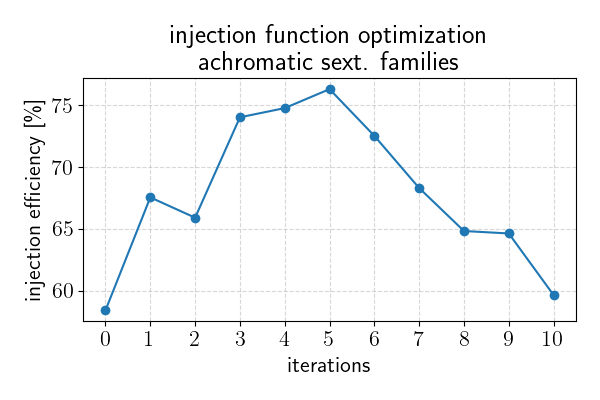
\includegraphics[width=0.7\columnwidth]{achromatic_fams_objective_func.png}
    \caption{Objective function vs iterations during the first run of injection efficiency optimization}
    \label{achrom_obj}
\end{figure}
We loaded the sextupole configurations found at iteration 5 and restored the nominal off-axis injection conditions. Injection efficiency fluctuated around 90-95\% with good repeatability. We measured coupling and found no difference from the usual value observed in the ref-config machine ($\sim$1\%). Beam-lifetime at 60~$\unit{mA}$ was about 21~hrs, which is 5~hrs smaller than lifetime at this current during users beam. The machine was cycled and the configurations from iteration 5 were loaded. Injection efficiency fluctuated at 90\%  and lifetime at 60~$\unit{mA}$ agreed with the 21 hrs observed previously.
\begin{figure*}[t]
    \centering
    \includegraphics*[width=\textwidth]{sexts_fams_configs.png}
    \caption{Sextupole families strengths and strength changes before/after the injection efficiency optimization using achromatic families}
    \label{achrom_sexts}
\end{figure*}

\section{Dynamic Aperture and Momentum Acceptance optimization}
Model simulations suggested that including an additional objective function to probe the momentum acceptance (MA) and the losses during Touschek scattering events could lead to a reduction in the impact of the DA optimization on lifetime. The RCDS objective function consisted on a scalar combination of both DA and MA objectives using adequate weights.
The DA objective was the off-axis injection efficiency at injection conditions mentioned early. The MA objective was the injection efficiency for a on-axis injection with a RF phase offset. The motivation for the latter conditions follows from the observation that beam-lifetime at SIRIUS is dominated by Touschek lifetime and the losses due to Touschek events occur at relatively small betatron actions ranging from 1--3~$\unit{\mu m}$, at energy deviations of 2--4\%. We aimed at replicating these conditions with a on-axis injection with a slight transverse and RF phase offsets to provide the beam with a small betatron action and to induce energy deviations in the aforementioned range. 
In the model, we found that using weight 1 for DA objective and weight 2 for MA objective worked well and usually led to DA improvements with some mild improvements of lifetime.

In the machine, the idea seemed not to work much. Figure~\ref{combined_obd} shows the combined objective function along the optimization iterations.  
\begin{figure}[h]
    \centering
    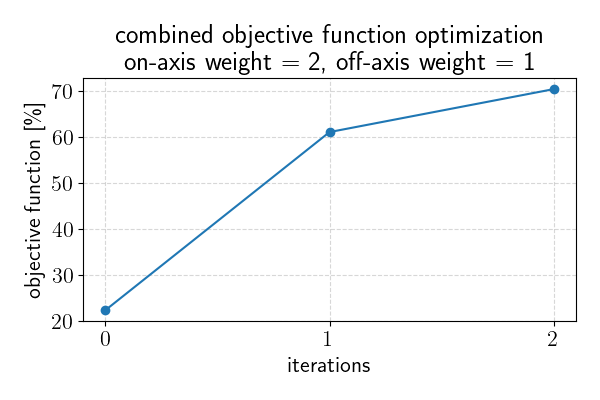
\includegraphics[width=0.7\columnwidth]{combined_objective_function.png}
    \caption{Objective function vs iterations during the first run of injection efficiency optimization}
    \label{combined_obd}
\end{figure}\textbf{}

\begin{figure*}[h]
    \centering
    \includegraphics*[width=\textwidth]{sexts_configs_combined_obj.png}
    \caption{Sextupole families strengths and strength changes before/after the combined objective function optimization}
    \label{combined_sexts}
\end{figure*}
\end{document}